\documentclass[preview]{standalone}

\usepackage{amsmath}
\usepackage{amssymb}
\usepackage{stellar}
\usepackage{definitions}

\begin{document}

\id{polynomials}
\genpage

\section{Polynomials}

% multiple indeterminates?
\begin{snippetdefinition}{polynomial-definition}{Polynomial}
    Let \((R, +, \cdot)\) be a ring.
    A \textit{polynomial} over \(R\) is an expression of the form
    \[
        p(x)=\sum_{k=0}^n a_n x^n
    \]
    where \(a_n\in R\) and \(x\) is an indeterminate.
\end{snippetdefinition}

\plain{Every polynomial induces a corresponding function.}

\begin{snippetdefinition}{polynomial-degree-definition}{Polynomial degree}
    Given a \polynomial of the form
    \[
        p(x)=\sum_{k=0}^n a_n x^n
    \]
    the \textit{degree} of \(p(x)\), denoted \(\deg p(x)\),
    is the maximum index \(k\) such that \(a_k \neq 0\).
\end{snippetdefinition}

\begin{snippet}{null-polynomial-expl}
    The polynomial \(p(x)=0\) has no degree. However, sometimes it is
    convenient to say that it has degree \(-\infty\) or \(-1\).
\end{snippet}

\section{Polynomial division}

\begin{snippettheorem}{polynomial-division-theorem}{Polynomial division}
    Let \(f(x)\) and \(g(x)\) be two \polynomial[polynomials] over \(R\)
    where \(g(x)\neq0\).
    Then, there always exist two unique polynomials \(q(x)\) and \(r(x)\) over \(R\)
    such that \[ f(x)=g(x)q(x) + r(x) \]
    where \(r(x)=0\) or \(\polynomialdeg r(x) < \polynomialdeg g(x)\).
\end{snippettheorem}

\begin{snippetproof}{polynomial-division-proof}{polynomial-division-theorem}{Polynomial division}
    \textbf{Existence di \(q(x)\) and \(r(x)\):} TODO
    \\
    \textbf{Uniqueness of \(q(x)\) and \(r(x)\):} TODO
\end{snippetproof}

\begin{snippet}{polynomial-division-method-illustration}
    \begin{center}
        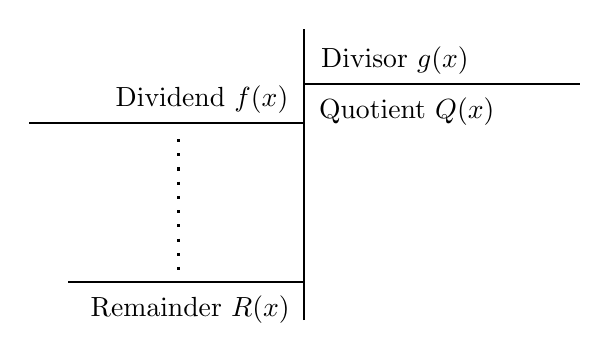
\begin{tikzpicture}
            %vline
            \draw[thick] (0,0) -- (0,3.7);
            %hlines
            \draw[thick] (0,3) -- (3.5,3);
            \draw[thick] (0,2.5) -- (-3.5,2.5);
            \draw[thick] (0,0.48) -- (-3,0.48);
            %dots
            \draw[line width=0.4mm, loosely dotted] (-1.6,2.3) -- (-1.6,0.6);
    
            %nodes
            \node at (1.15,3.3) {Divisor $g(x)$};
            \node at (-1.3,2.8) {Dividend $f(x)$};
            \node at (1.3,2.65) {Quotient $Q(x)$};
            \node at (-1.45,0.13) {Remainder $R(x)$};
        \end{tikzpicture}
    \end{center}
\end{snippet}

%\begin{snippetcorollary}{polynomial-divisibility-by-x-1}{Polynomial divisibility by \(x-1\)}
%    Let
%    \[ P(x) = \sum_{k=0}^n a_k x^k \]
%    be a \polynomial. Then, \(P(x)\)
%    is divisible by \(x-1\) if
%    \[ \sum_{k=0}^n a_k = 0 \]
%\end{snippetcorollary}

\end{document}